\documentclass[letterpaper,spanish,11pt]{article}
\usepackage[utf8]{inputenc}    % Agregar y acentos
\usepackage{babel}               % Soporte multilenguajes
%\usepackage{avant}               % Tipo de fuente
%\usepackage{fancyheadings}       %% Topes y pies de p�ina
%\usepackage[dvips]{graphicx}     % Inclusion de imagenes .eps
\usepackage{amsmath,amsthm,url}
%\usepackage{url}                 % Agregar Links soporte de ~
\usepackage{verbatim}
%\usepackage{geometry}
\usepackage{color}
\usepackage{amsfonts}
\usepackage{amssymb}
%\usepackage{txfonts}
%\usepackage{pxfonts}
%\usepackage{fancybox}
\usepackage{latexsym}
%\usepackage{fancyvrb}
\usepackage{graphicx}
%\usepackage{pstricks}
\usepackage{setspace} % paquete para interlineado
\usepackage{url}
\usepackage{colortbl}
\usepackage{multirow}
\usepackage{slashbox}
\usepackage{rotating}
\definecolor{rojo}{rgb}{1,0,0}
\oddsidemargin -0.1in
\topmargin -0.5in
\textwidth 6.7in
\textheight 8.5in

\begin{document}

\begin{titlepage}
%\begin{figure}[htbp]
\begin{center}

\includegraphics[height=3.5cm]{images/logo_latex}  %se coloca solo el nombre de archivo sin .extension y la imagen en formato .png
\end{center}
%\end{figure}
\vspace{1.5cm}
\begin{center}
\textbf{\Huge{Laboratorio de estad\'istica}}\\[0.2cm]
\textbf{\Huge{computacional}}\\[0.7cm]
\textbf{\huge{Informe \# 2}}\\[0.7cm]
\textbf{\huge{``Regresi\'on Lineal Simple''}}\\[0.3cm] % en caso de que el titulo del tema sea corto, ajustar las medias para que los nombres de los integrantes queden mas abajo
\today\\[1.5cm]
\end{center}
\vspace{3cm}
\begin{flushright}
\large{\textbf{Profesor de C\'atedra}} \\
\large{Ricardo \~{N}anculef} \\[0.5cm]
\large{\textbf{Ayudantes de laboratorio}}\\
\large{Milciades Reyes}\\
\large{Fernando Herrera}\\[0.5cm]
\large{\textbf{Integrantes}} \\
\large{Esteban Bombal 2673004-k} \\
\large{Rodrigo Fernandez 2673002-3} \\
\large{Cristian Maureira 2673030-9} \\
\large{Gabriel Zamora 2673070-8} \\
\end{flushright}
\end{titlepage}

\section*{Descripci\'on del Fen\'omeno y del Muestreo}

\begin{enumerate}
	\item \emph{Hipotesis:} El puntaje que las personas obtienen en la prueba de seleccion universitaria,
			 no representa el desempeño que tendran en la universidad.
	\item \emph{Variables:}
		\begin{itemize}
			\item Puntaje Psu \emph{(continua)}
			\item Prioridad Acad\'emica \emph{(continua)}
			\item A\~nos que lleva en la universidad \emph{(discreta)}
		\end{itemize}
	\item \emph{Metodolog\'ia de muestreo:}
	\begin{enumerate}
		\item Poblaci\'on Objetivo:
				Alumnos de la Universidad T\'ecnica Federico Santa Mar\'ia
		\item Muestra:
				Alumnos de la Casa Central
		\item Marco Muestral:
				Estudiantes de Inform\'atica, Industrias, Qu\'imica, Obras Civiles.
		\item Metodolog\'ia utilizada:
				No-Aleatorizado y por conveniencia.
		\item Justifiaci\'on del porque elegimos esta metodolog\'ia:
				%esta es la misma metodologia que el informe anterior, hay que cambiarle las palabras
       				Principalmente, fue por el gasto en tiempo que significaba el realizar una encuesta de otro tipo.\\
				Tambien encontramos que, subjetivamente, las distintas personas encuestadas que logramos contactar 
				fueron lo suficientemente variadas como para representar una porci\'on considerable de la poblaci\'on.
	\end{enumerate}


\end{enumerate}

\section*{Regresi\'on lineal Simple}
\label{sec:rls}
%elija una variable cuantitativa continua, la cual va a ser dependiente en el analisis
%y otra variable cuantitativa continua, la cual va a ser independiente
%primera parte: dependiente(y): prioridad, independiente(x): psu
\begin{enumerate}
	\item Calcular:\\
	\textbf{x:} variable independiente (puntajes psu)\\
	\textbf{y:} variable dependiente (prioridad acad\'emica)
	\begin{itemize}
		\item Covarianza:
			$$cov(x,y)\ =\ \frac{1}{n}\sum_{i=1}^{n}{(x_{i}-\bar{x})\cdot(y_{i}-\bar{y})}\ =\ 21379.98$$
		\item Coeficiente de correlaci\'on:
			$$\rho_{xy}\ =\ \frac{cov(x,y)}{\sigma_{x}\sigma_{y}}\ =\ 0.2780022$$
		\item Coeficiente de la recta de regresi\'on:
			$$\bar{y}\ =\ a\ +\ b\bar{x}$$
			$$b\ =\ \frac{cov(x,y)}{var(x)}\ =\ 12.23432$$
		\item Desviaci\'on t\'ipica generalizada:
			$$M\ =\ \left[ \begin{array}{lr}
		            S_{x}^{2}      &  \rho S_{x}S_{y}  \\
		            \rho S_{x}S_{y} &  S_{y}^{2}  
		           \end{array}
			    \right]
			$$
			$$|M|^{1/2}\ =\ S_{x}S_{y}\sqrt{1-\rho^{2}}$$

			Como:
			$$\sigma_{x}\ =\ 41.80359$$
                       	$$\sigma_{y}\ =\ 1839.693$$
			$$\rho \ =\ 0.2780022$$
			$$|M|^{1/2}\ =\ 73874.1771244$$
			
		\item Gr\'afico de dispersi\'on con la recta de regresi\'on:
			\begin{center}
                        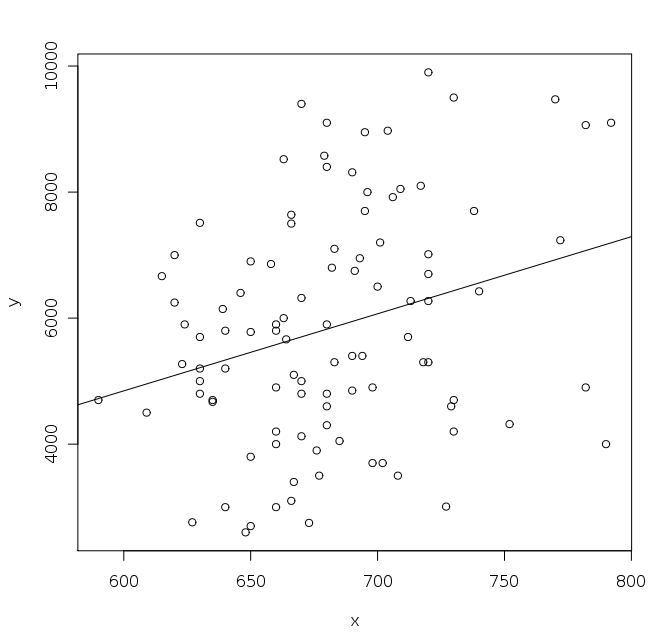
\includegraphics[width=4in]{images/grafico_dispersion1.png}
			\end{center}

	\end{itemize}
	\item Calcular:
	\begin{itemize}
		\item Media:
			$$Media_{errores}\ =\ 3.874873e-14$$
		\item Varianza de los errores:
			$$Var_{errores}\ =\ 3122900$$
	\end{itemize}
	\item Gr\'aficos:
	\begin{itemize}
		\item Diagrama de Caja:
			\begin{center}
                        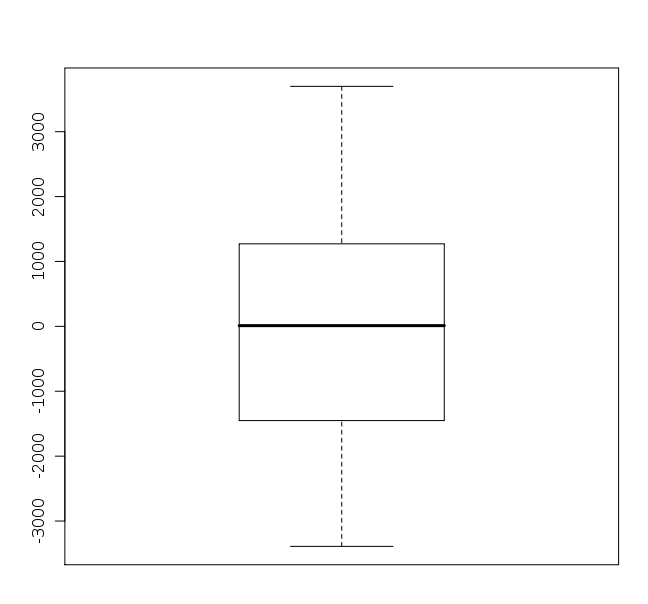
\includegraphics[width=4in]{images/boxplot1.png}
			\end{center}
		\item Histograma de los errores:
			\begin{center}
                        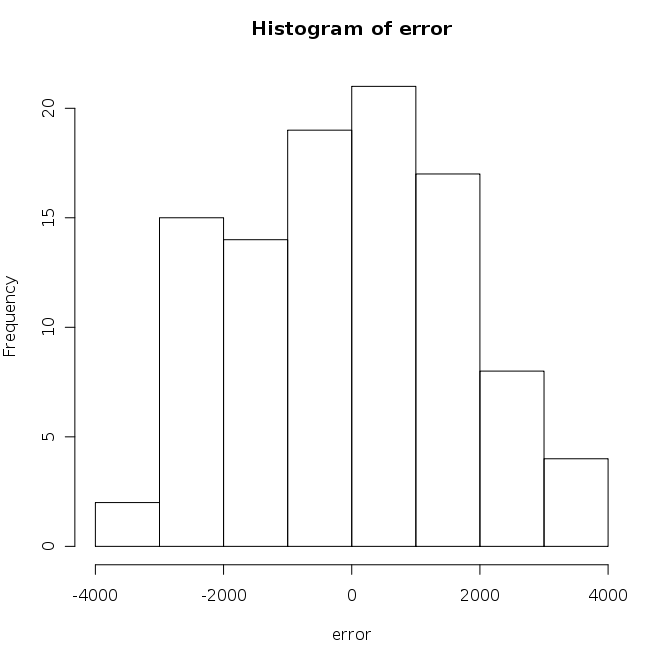
\includegraphics[width=4in]{images/hist1.png}
			\end{center}
	\end{itemize}
	\item Conclusiones:
		Podemos ver claramente, que no existe ninguna relaci\'on entre el puntaje de la Prueba de Selecci\'on Universitaria y la Prioridad Acad\'emica que poseen los alumnos encuestados.
		Atribuimos \'esta falta de relaci\'on porque el nivel y la metodolog\'ia de ense\~nanza que existe en los distintos colegios no es la misma, hay establecimientos educacionales
		que se preocupan de preparar a sus alumnos s\'olo para que tengan un buen rendimiento en la PSU, otros para que tengan un buen rendimiento en la Universidad y algunos pocos
		para que se desempe\~nen bien en ambos lugares, por lo tanto es muy comun que la mayor\'ia de las personas que entran a la universidad con los mejores puntajes, tienen un
		rendimiento desfavorable, a pesar que existen las excepciones. Otro punto importante, es que dependiendo de la cantidad de a\~nos que llevan en la Universidad, pueden haber
		surgido problemas de otro tipo que no sean acad\'emicos que pudiesen influir en un mal desempe\~no al cursar los ramos.
		Si lo vemos de forma m\'as aplicada podemos darnos cuenta que el coeficiente de correlaci\'on se acerca mucho a $0$ y bien sabemos que si $-1 < \rho < 1$, no existe relaci\'on
		lineal exacta.

	%comente sobre los resultados obtenidos en las preguntas anteriores
	\item ?`Es necesario realizar una transformaci\'on a los datos para obtener
		una relaci\'on lineal?

		Analizando los graficos de dispersi\'on, podemos ver que los datos no presentan una relaci\'on lineal, lo que se se\~nala en el punto anterior. Tampoco es posible encontrar algun tipo de relaci\'on tanto logar\'itmica, estad\'istica o alguna otra, por lo que realizar alg\'un tipo de transformaci\'on para lograr una regresi\'on lineal ser\'ia in\'util.\\

	\item  Calcule y compare $\beta_{0}^{'}$ con  $\beta_{0}^{''}$ y $\beta_{1}^{'}$
		con  $\beta_{1}^{''}$ \\ \\
			$\widehat{y} = \beta_0 + \beta_1 x$ \\
			$\Leftrightarrow \widehat{y} = -2495.00 + 12.23 x$ \\
			$\Leftrightarrow \widehat{x} = \frac{y}{\beta_1} - \frac{\beta_0}{\beta_1}$ \\
			$\Leftrightarrow {\beta_1}' = 1/\beta_1 \ \ \ \ {\beta_0}' = -\beta_0/{\beta_1}$ \\
			$\Leftrightarrow {\beta_1}' = 0.08176615 \ \ \ \ {\beta_0}' = 204.0065$ \\ \\

			$\widehat{x} = {\beta_0}'' + {\beta_1}'' y$ \\
			$\Leftrightarrow {\beta_0}'' = 645 \ \ \ \ {\beta_1}'' = 0.006317$ \\ \\

			Claramente se observa que tanto ${\beta_1}'$ y ${\beta_1}''$ como ${\beta_0}'$ y ${\beta_0}''$ respectivamente, poseen valores completamente diferente. Esto se produce debido a que estas constantes  ${\beta_1}'$ y ${\beta_0}'$ se modelaron mediante una fracci\'on entre constantes que fueron calculadas mediante la diferencia vertical de las variables con la recta de regresi\'on, por otro lado las constantes ${\beta_1}''$ y ${\beta_0}''$ fueron modeladas segun diferencias horizontales de las variables con respecto a la recta de regresi\'on.\\

	\item Agregando un dato at\'ipico:
			
			$\beta_0 = 728.49 \ \ \ \ \beta_1 = 7.65$ \\ \\
			\begin{center}
			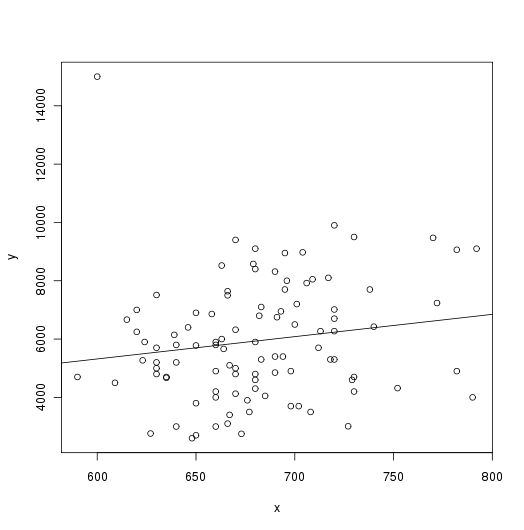
\includegraphics[width=4in]{images/grafico_dispersion1_dato_atipico.png}
			\end{center}

			Comentarios: \\ \\
			Podemos ver claramente que la recta de regresi\'on se ve afectada de manera importante, con la presencia del dato at\'ipico, lo que llev\'o a modificar los coeficientes que la defin\'ian, disminuyendo notoriamente la ya m\'inima predicci\'on que la recta prove\'ia de los datos. \\

	\item Repitiendo los puntos 1, 2, 3, 4 y 5, tomando como variable independiente
		la otra variable cuantitativa discreta
%segunda parte: dependiente(y): prioridad, independiente(x): a�os de estudio%
		\begin{enumerate}
			\item Calcular:
				\begin{itemize}
				\item Covarianza:
					$$cov(x,y)\ =\ \frac{1}{n}\sum_{i=1}^{n}{(x_{i}-\bar{x})\cdot(y_{i}-\bar{y})}\ =\ -232.3434$$
				\item Coeficiente de correlaci\'on:
					$$\rho_{xy}\ =\ \frac{cov(x,y)}{\sigma_{x}\sigma_{y}}\ =\ -0.07456646$$
				\item Coeficiente de la recta de regresi\'on:
					$$b\ =\ \frac{cov(x,y)}{var(x)}\ =\ -80.99296$$
					$$\bar{y}\ =\ 6123.33\ -\ 80.99\cdot\bar{x}$$
				\item Desviaci\'on t\'ipica generalizada: 
					$$M\ =\ \left[ \begin{array}{lr}
			        	S_{x}^{2}      &  \rho S_{x}S_{y}  \\
			  		\rho S_{x}S_{y} &  S_{y}^{2}  
				        \end{array}
					\right]
					$$
					$$|M|^{1/2}\ =\ S_{x}S_{y}\sqrt{1-\rho^{2}}$$

					Como:
			               	$$\sigma_{x}\ =\ 1839.693$$
					$$\sigma_{y}\ =\ 1.69372$$
					$$\rho \ =\ -0.07456646$$
						$$|M|^{1/2}\ =\ 3230.008$$


		%			$$sd(x)=\ 1839.693$$
				\item Gr\'afico de dispersi\'on con la recta de regresi\'on:\\
				\begin{enumerate}
					\item Gr\'afico de dispersi\'on del tiempo de permanencia en la universidad versus la prioridad actual del estudiante:\\
			  	  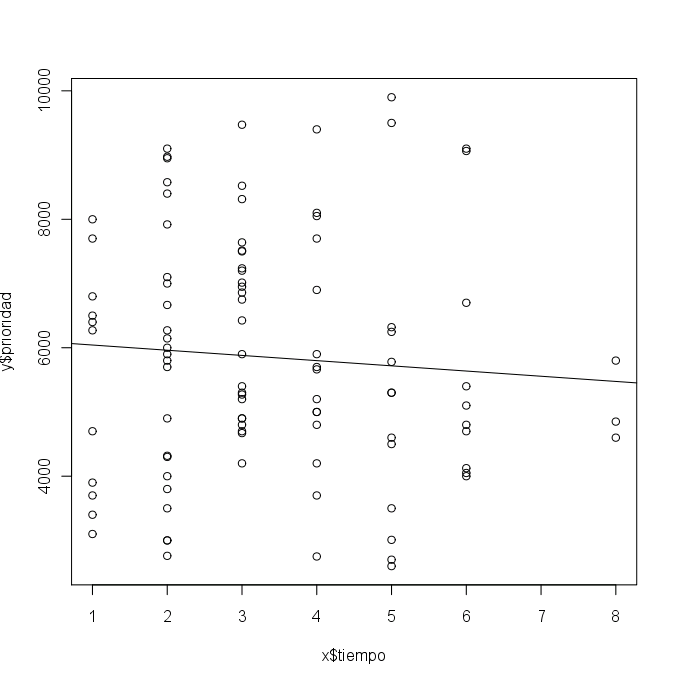
\includegraphics[width=4in,height=4in]{images/plot_2-1.png}
					\item Gr\'afico de dispersi\'on del tiempo de permanencia en la universidad versus la prioridad actual del estudiante, pero agrupando con las medias de las mediciones:\\
			  	  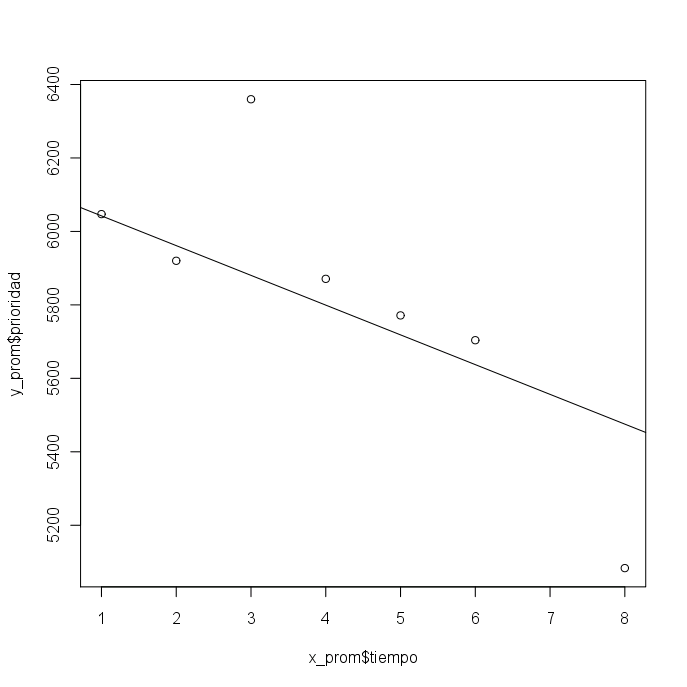
\includegraphics[width=4in,height=4in]{images/plot_2-3.png}
				\end{enumerate}
				\end{itemize}
			\item Calcular:
				\begin{itemize}
				\item Media de los errores obtenidos:
%				> mean(abs(errores))
% 				$$ 1492.753 $$
%				> mean(errores)
				$$Media(errores)\ =\ 3.648776e-14$$
				$$Media(errores)\ ~ 0$$
				\item Varianza de los errores:
%				> var(errores)
				$$S^2(errores)\ =\ 3365652$$
				\end{itemize}
			\item Gr\'aficos:
				\begin{itemize}
				\item Diagrama de Caja:\\
			  	  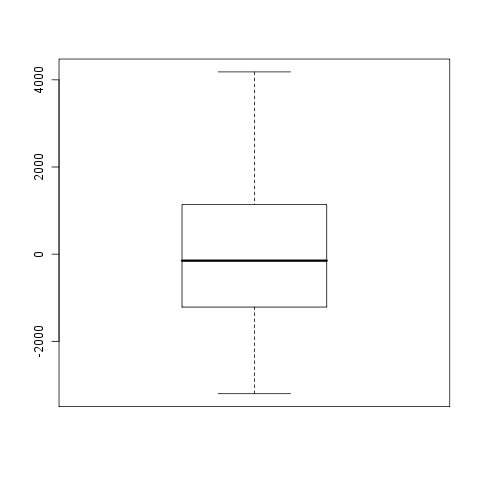
\includegraphics[width=4in,height=4in]{images/2_boxplot}
				\item Histograma de los errores:\\
			  	  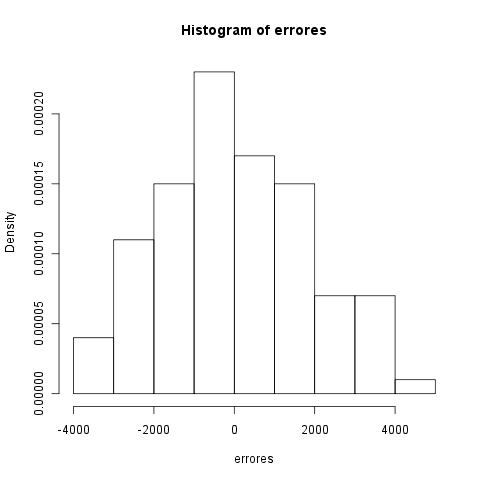
\includegraphics[width=4in,height=4in]{images/2_histogram}
				\end{itemize}
			\item Conclusiones:\\
			%comente sobre los resultados obtenidos en las preguntas anteriores
			Se puede notar que existe una especie de patron entre las variables, pero se dificulta un poco
			la visibilidad de esta por la variabilidad en la cantidad de mediciones por cada a\~no de estancia
			en la universidad (es dificil encontrar para encuestar a muchos de los ultimos a\~nos, por lo que la
			poca cantidad de mediciones genera distorciones en la curva de correlaci\'on lineal). Aun as\'i,
			concluimos que, a pesar de que no se ve a simple vista, las variables de la prioridad acad\'emica y la
			cantidad de a\~nos que uno lleva en la universidad si estan relacionados, y esa relaci\'on toma una
			forma que se puede explicar linealmente. Esto se ve mucho mas claro al estratificar por a\~no academico,
			tomando en cuenta solo los promedios de las prioridades de cada uno. Este decrecer de la prioridad puede
			darse por variados factores, por lo que se deberian realizar mas analisis para ver si esta aparente baja
			de notas se deba a la desmotivaci\'on academica de los estudiantes o al aumento de la dificultad de ciertos
			ramos de \'ultimo a\~no.
			\item ?`Es necesario realizar una transformaci\'on a los datos para obtener
				una relaci\'on lineal? \\
				En el punto anterior se~nalamos que no era necesario realizar alguna transformaci\'on a los datos, ya que pudimos establecer una relaci\'on lineal entre ellos.
		\end{enumerate}
	\item ?`Qu\'e variable independiente est\'a m\'as relacionada con la variable dependiente?
		En nuestro caso, la cantidad de a\~nos de estudio tiene una relacion mucho mayor con la prioridad que el puntaje PSU
		con la variable dependiente, ya que en la mayor\'ia de los casos, la prioridad va disminuyendo a medida que pasan los
		a\~nos, \'esto tiene mucha relaci\'on con la f\'ormula con la cual se calcula, y tambien porque la dificultad de los
		ramos va aumentando, entonces el desempe\~no de un alumno de primer a\~no es muy distinto al de un alumno de sexto a\~no
		que aparte de ``pasar ramos'', posee otras responsabilidades, impartir ayudantias, trabajos, proyectos, etc.
		Podemos tambi\'en darnos cuenta de cual variable independiente esta mucho mas relacionada con la variable dependiente
		mirando el \emph{coeficiente de correlaci\'on}, en el caso de la PSU, $\rho \approx 0.27$ y en el caso de los a\~nos
		que los estudiantes llevan en la universidad $\rho \approx -0.07$, entonces claramente la PSU obtiene un poco mas de relaci\'on
		esto se debe a que es mucho mas certero decir \emph{a medida que pasan los a\~nos, la prioridad baja porque la cantidad de cr\'editos
		va disminuyendo, o por la misma f\'ormula que calcula la prioridad}, que decir \emph{si el puntaje en la PSU es mayor, mayor la prioridad}.

\end{enumerate}



\section*{Preguntas Optativas}
\label{sec:optativas}
	%Teniendo la variable cuantitativa discreta como independiente, se tienen varios
	%valores de y_{i} para un valor de x_{j}, realice los siguientes puntos
	\begin{enumerate}
		\item Calcular:
			\begin{itemize}
			\item Promedios de $y_{i}$ que corresponden a un $x_{j},\ \forall\ i,j$ \\ \\
			En nuestro caso, tomamos $y_i = $ A~nos que lleva en la universidad (discreta) y por conveniencia tomamos $x_j = $ Prioridad Acad\'emica.\\
			Entonces, calculamos los promedios de $x_j$ para cada $y_i$ y obtenemos la siguiente tabla:\\ \\
			\begin{tabular}{c|c}
			\hline
			A\~nos en la Universidad & Promedio Prioridad Acad\'emica \\
			\hline
			1 & 5497,36 \\
			\hline
			2 & 5920,04 \\
			\hline
			3 & 6359,83 \\
			\hline
			4 & 5870,86 \\
			\hline
			5 & 5327,38 \\
			\hline
			6 & 5703,80 \\
			\hline
			7 & 0000,00 \\
			\hline
			8 & 5083,33 \\
			\hline
			\end{tabular}
			\item Covarianza: $ -2500.714 $
			\item Coeficiente de correlaci\'on: $ -0.4989711 $
			\item Coeficientes de la recta de regresi\'on: $y\ =\ b_{1} \cdotp x\ +\ b_{0}$, $y\ =\ -416.8 \cdotp x\ +\ 6845.9 $
			\item Desviaci\'on t\'ipica generalizada: $1915$
			\item Media: 4970,32791
			\item Varianza de los errores: $Error\ b_{1}\ =\ 295.5$, $Error\ b_{0}\ =\ 1492.3 $
			\end{itemize}
		\item Gr\'aficos:
			\begin{itemize}
			\item Dispersi\'on con la recta de regresi\'on:
			\begin{center}
			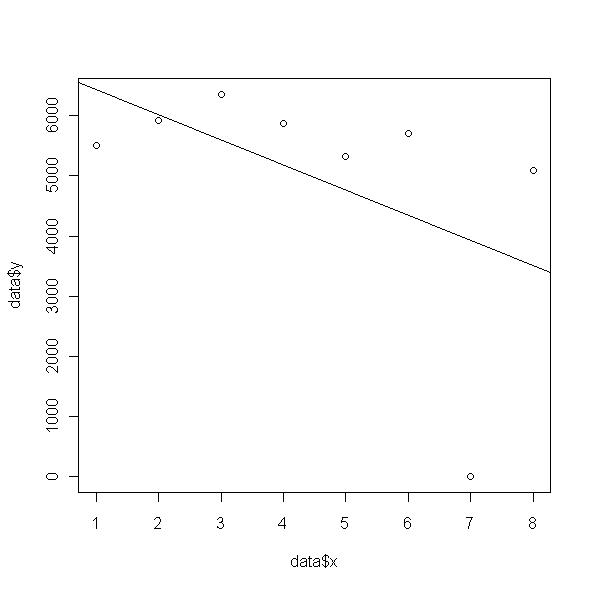
\includegraphics[width=4in,height=4in]{images/grafico_dispersion_optativo}
			\end{center}
			\item Diagrama de caja:
			\begin{center}
			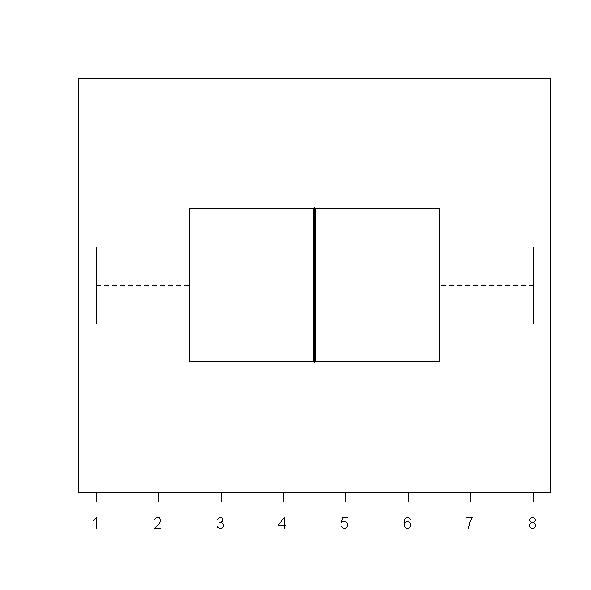
\includegraphics[width=4in,height=4in]{images/boxplot}
			\end{center}
			\item Histograma de los errores:
			\begin{center}
			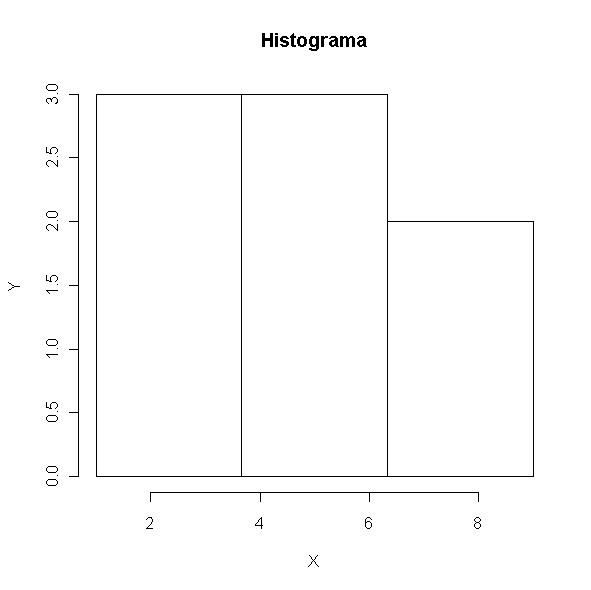
\includegraphics[width=4in,height=4in]{images/histograma}
			\end{center}
			\end{itemize}
		\item Conclusi\'on:
			Como podemos observar en la recta de regresi\'on, al parecer si existe una relaci\'on entre las variables,
			espec\'ificamente una relaci\'on inversamente proporcional entre los a~nos de estad\'ia en la Universidad
			T\'ecnica Federico Santa Mar\'ia y la Prioridad Acad\'emica del alumno. Posiblemente porque seg\'un est\'a
			dada la ecuaci\'on para calcular este coeficiente, es mucho mas dificil para el alumno aumentarlo que disminuirlo,
			lo cual queda demostrado, por la cantidad de gente que tiene que irse de la universidad por tener una prioridad
			muy baja, ya que los ramos de los primeros a\~nos son claves para poder tener una buena prioridad de base, tomando
			en cuenta que mas adelante el grado de dificultad de los ramos aumenta y hay mucha m\'as probabilidad de reprovar
			algun ramo y como los cr\'editos no son tantos, subir la prioridad acad\'emica es a\'un mas dificil.
	\end{enumerate}


\end{document}
